
\section{System Level Structural Diagram (Block Diagram)} % pending 
\label{sec:block}


\begin{figure}[htbp]
\begin{center}
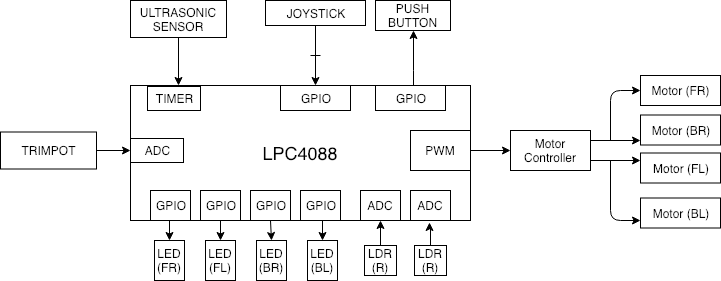
\includegraphics[width=1\columnwidth]{figures/443-Diagram-block.png}
\end{center}
\caption{Block Diagram of car.}
\vskip\baselineskip % Leave a vertical skip below the figure
\label{fig:sample}
\end{figure}

\textbf{LPC4088 Microcontroller:} Main part of the car. Runs software and controls peripherals.

\textbf{Motor controller:} By getting inputs from the main board, controls motors by means of controlling speed, directions, soft and hard brakes.

\textbf{Motor:} Gives tork to the car, and thus moves.

\textbf{LEDs:} Emits light, controlled by the main board. Used for car signals.

\textbf{Joystick:} Takes input from the player/user and informs the main board, so it can take appropriate action.


\textbf{Push Button:} It is used to toggle mode to Manuel and Auto with interrupts. 

\textbf{Ultrasonic sensor:} Car can measure distance with ultrasonic sensor. 

\textbf{Trimpot:} Used to adjust motor speed. It can take value between 0-100. 
